\chapter{Ensemble Learning}
\begin{description}
    \item[Combining Base Learners]Multiexpert combination method: base learners
        work in parallel, give decision and combined to give a final.

        Multistage combinations: Base learners work serially, sorted increasing
        complexity, complex is used when simple is not confident.
    \item[Voting] Takes a convex combination of the base learners:\[
        y = f(d_1, \dots, d_L|\bPhi) = \sum_{j=1}^L w_j d_j(\bx)\], with
        $w_j \geq 0$ and $\sum_{j=1}^L w_j = 1$, $\bPhi = (w_1, \dots,
        w_L)^T$ are the parameters and $y$ is the final prediction.
    \item[Voting for Classification] for class $C_i$ $y_i = \sum_{j=1}^L w_j
        d_{ij}(\bx)$, where $d_{ij}$ is the vote of learner $j$ for $C_i$

        Simple voting $w_j = \frac{1}{L}$

        Bayesian model combination: $P(C_i|x) = \sum_{models
            \mathcal{M}_j}P(C_i|x, \mathcal{M}_j)P(\mathcal{M_j})$, weight $w_j$
            can be seen as approximation of the prior $P(\mathcal{M}_j)$,
            Analysis, as $L$ increase, bias does not change but the variance
            decreases.
    \item[Bagging] bootstrap aggregation, a voting method whereby the base
        learners are made different by training on slightly different training
        sets.
    \item[AdaBoost] Modifies the probabilities of drawing instances for
        classifier training as a function of the error of the previous base
        learner.
        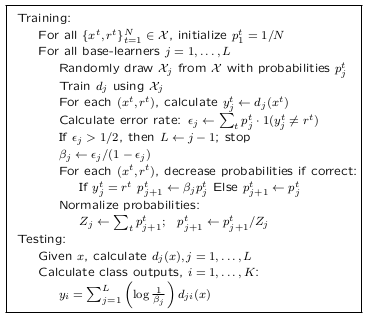
\includegraphics[width=14cm]{alg}


\end{description}
\section{Matrices Properties}
\begin{description}
    \item[Basic Matrix]
        $(\bA\bB)^T = \bB^T\bA^T$, 
    $(\bA\bB)^{-1} = \bB^{-1}\bA^{-1}$, $(\bA^T)^{-1} = (\bA^{-1})^T$, 
    $\mathbf{P}^{-1}+\bB^T \bR^{-1}\bB)^{-1}\bB^T\bR^{-1} = \mathbf{P}\bB^T(\bB
    \mathbf{P}\bB^T+\bR)^{-1}$, 
\item[Traces and Determinants] $Tr(\bA\bB) = Tr(\bB\bA)$, $Tr(\bA\bB\bC) = Tr(\bC\bB\bA) = Tr(\bB\bC\bA)$,
    $|\bA^{-1}| = \frac{1}{|\bA|}$, $\ba^T\bA\ba = Tr(\bA \ba\ba^T)$
\item[Matrix Derivatives] $\frac{\partial}{\partial \bx}(\bx^T\ba) =
    \frac{\partial}{\partial \bx}(\ba^T\bx) = \ba$,
    $\frac{\partial}{\partial\bx}(\bA\bB) = \frac{\partial \bA}{\partial \x}\bB
    +\bA\frac{\partial \bB}{\partial \bx}$, $\frac{\partial}{\partial
    x}(\bA^{-1}) = -\bA^{-1}\frac{\partial \bA}{\partial x}\bA^{-1}$, 
    $\frac{\partial}{\partial x}\ln |\bA| = Tr(\bA^{-1}\frac{\partial
    \bA}{\partial x})$, $\frac{\partial}{\partial A_{ij}}Tr(\bA\bB) = B_{ji}$,
    $\frac{\partial}{\partial \bA}Tr(\bA\bB) = \bB^T$, $\frac{\partial}{\partial
    \bA}Tr(\bA) = \mathbf{I}$, $\frac{\partial}{\partial \bA}Tr(\bA\bB\bA^T) =
    \bA(\bB+\bB^T)$, $\frac{\partial}{\partial \bA}\ln |\bA| = (\bA^{-1})^T$
\end{description}

